\documentclass[12pt]{beamer}

% Pakete
\usepackage[utf8]{inputenc}
\usepackage[german]{babel}

% AMS Pakete
\usepackage{amsmath}
\usepackage{amsfonts}
\usepackage{amssymb}

\usepackage{braket}

% Einheiten
\usepackage{siunitx}
\sisetup{
	output-decimal-marker={,},
	separate-uncertainty
}

% Grafiken
\usepackage{graphicx}


% Theme
\usetheme{Boadilla}
\usecolortheme{rose}
\useoutertheme{infolines}
\useinnertheme{rectangles}
\usefonttheme[onlymath]{serif}

% [num] Zitationen
\setbeamertemplate{bibliography item}[text]

% Navigationsleiste ausschalten
\beamertemplatenavigationsymbolsempty

\DeclareMathOperator{\divergence}{div}

\author[Christopher Deutsch]
{Christopher Deutsch}

\title
{Atomfallen}

\subtitle
{Überblick über die Funktionsweise der wichtigsten Fallen}
%\logo{}

\institute[]
{Rheinische Friedrich-Wilhelms-Universität Bonn \\
Proseminar Präsentationstechnik SS15}

\date{8. Juni 2015}

%\setbeamercovered{transparent}
%\setbeamertemplate{navigation symbols}{}

\begin{document}
\maketitle

\begin{frame}{Inhalt}
	\tableofcontents
\end{frame}


\section{Motivation}

\begin{frame}{Was sind Atomfallen?}
	\begin{itemize}
		\item Teilchen die durch eine ortsabhängige Kraft in einem Raumvolumen eingeschlossen werden
		\item Suspend matter without material walls
		\item Minimaler Einfluss auf die innere Struktur
		\item Minimale Heizung durch die Umgebung
		\item Beobachtung von einzelnen Atomen über längere Zeit
	\end{itemize}
\end{frame}

\begin{frame}{Grundlagen}
	\begin{itemize}
		\item Fallenpotential und Tiefe
		\begin{align}
		\Delta E = k_\mathrm{B} \cdot T
		\end{align}
		\item Temperatur der Teilchen (Raumtemperatur $\approx \frac{1}{40} \si{eV}$)
		\item Köhlung?
		
	\end{itemize}
	\begin{figure}
		\centering
		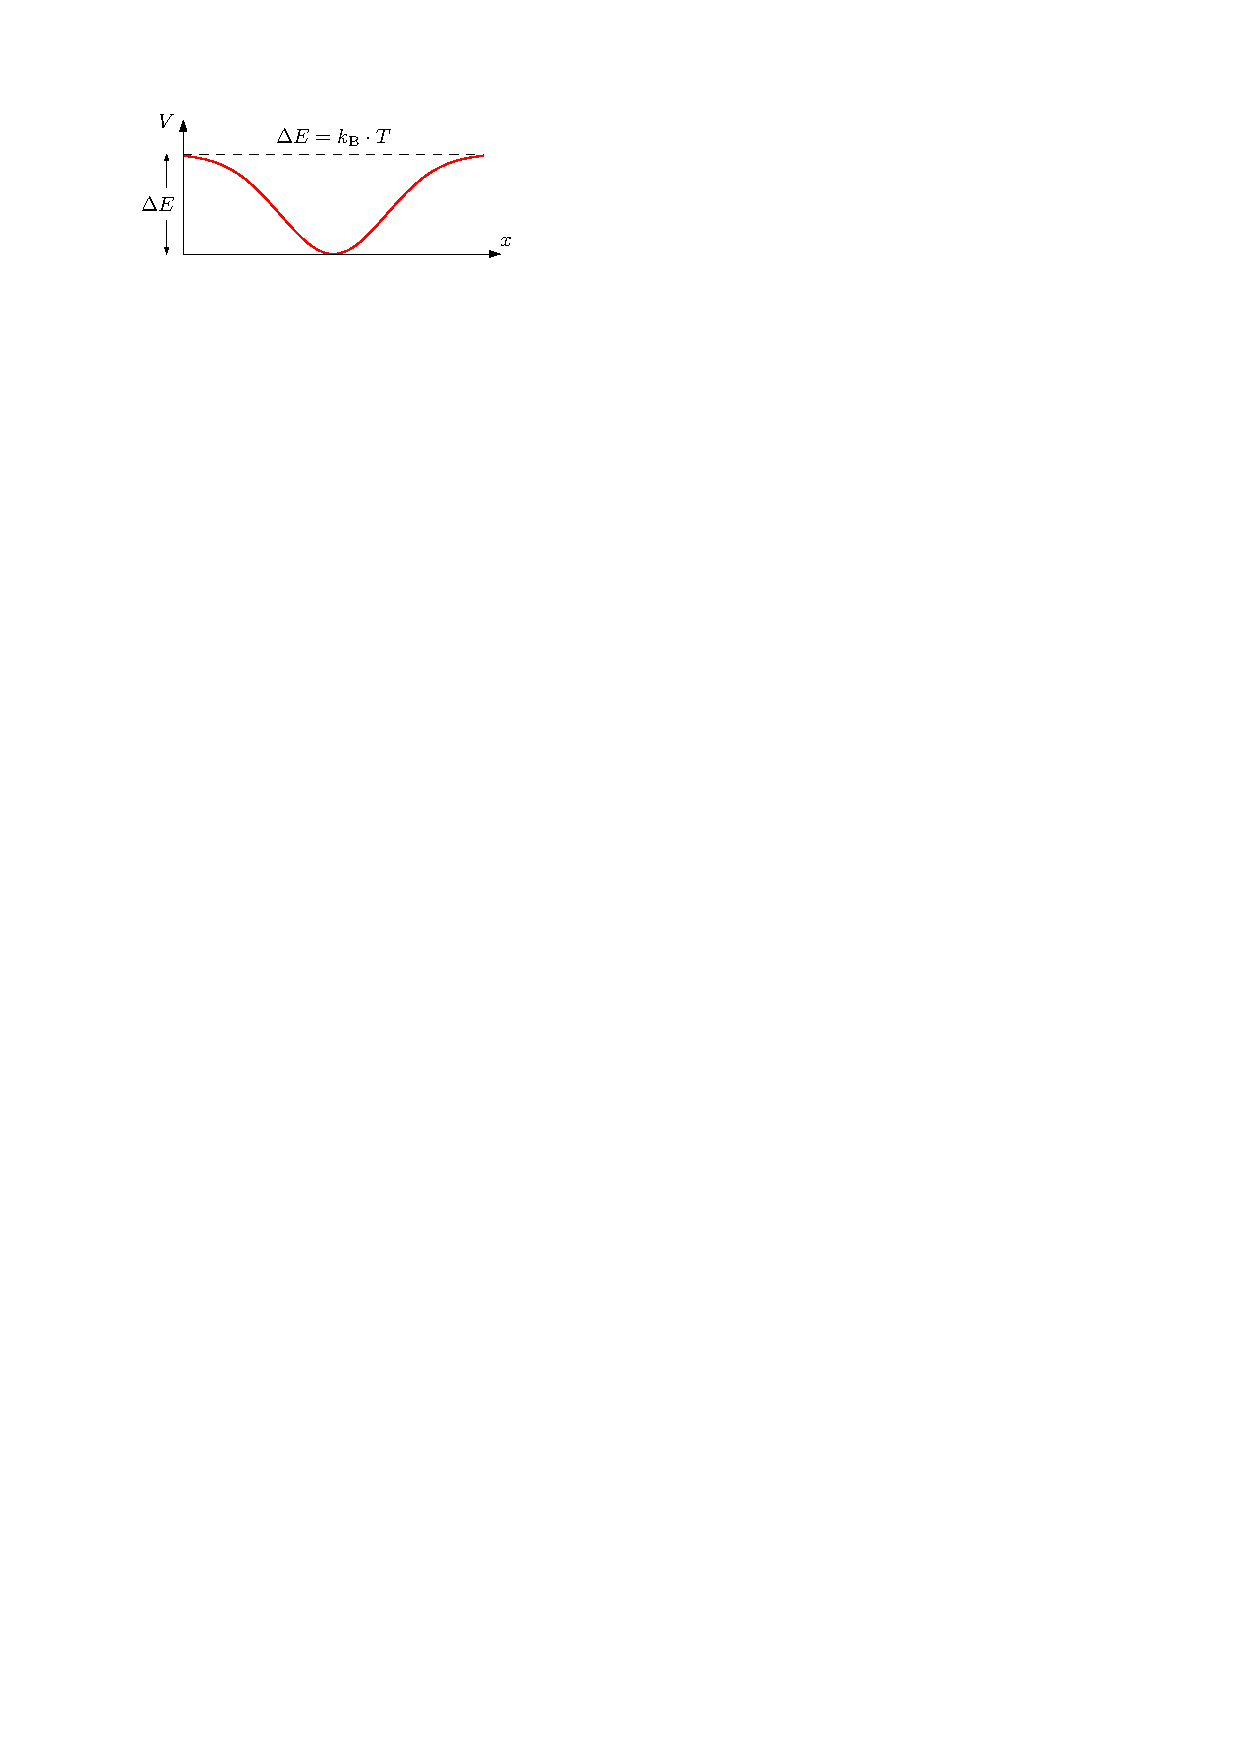
\includegraphics[width=0.6\textwidth]{./figures/fallentiefe.pdf}
	\end{figure}
\end{frame}

\begin{frame}{Wofür braucht man Atomfallen?}
	\cite{wpw}:
	\begin{itemize}
		\item BEC (niedrige Temperaturen)
		\item High-Resolution-Spectroscopy (Dopplereffekt, Zeitdilatation vermieden)
		\item Atomuhren (NP 1989 Ramsey, Paul, Dehmelt) (Auch Spektroskopie)
		\item Quantencomputer (Qubit)
		\item Quantum measurements on single atoms
		\item Quantum-state engineering
	\end{itemize}
\end{frame}


\section{Ionenfallen}

\begin{frame}{Grundlagen der Ionenfallen}
	\begin{itemize}
		\item Kraft auf geladene Teilchen groß (EM-WW ist stark)
		\item Große Fallentiefen (Keine Kühlung nötig) Teilchen können direkt in der Falle ionisiert werden
		\item typische Fallentiefen: $\SI{6e6}{\kelvin}$ bei Betriebsspannung \SI{500}{V}
	\end{itemize}
\end{frame}



\begin{frame}
	1. Maxwell-Gleichung für den ladungsfreien Raum (Quellenfreiheit):
	\begin{align}
	\divergence \vec{E} = 0
	\end{align}
	\begin{align}
	\int_{V} \divergence \vec{E} \, \mathrm{d}V = \oint_{S = \partial V} \vec{E} \cdot \vec{n} \, \mathrm{d}S = 0
	\end{align}
	

\end{frame}

\begin{frame}
	Fangen eines positiven Ions in einem Raumvolumen: $\vec{E} \cdot \vec{n} \stackrel{!}{<} 0$
	\begin{figure}
		\centering
		\includegraphics*[width=0.5\textwidth]{./figures/earnshaw.pdf}
	\end{figure}
		\begin{block}{Earnshaw-Theorem:}
			Ein geladenes Teilchen kann nicht durch elektrostatische Kräfte in einem Raumvolumen gefangen werden.
		\end{block}
\end{frame}

\begin{frame}{Lineare Paul-Falle ($x$-$y$-Ebene)}
	\begin{columns}[t]
		\column{0.5\textwidth}
		Quadrupol:
		\begin{figure}[h]
			\centering
			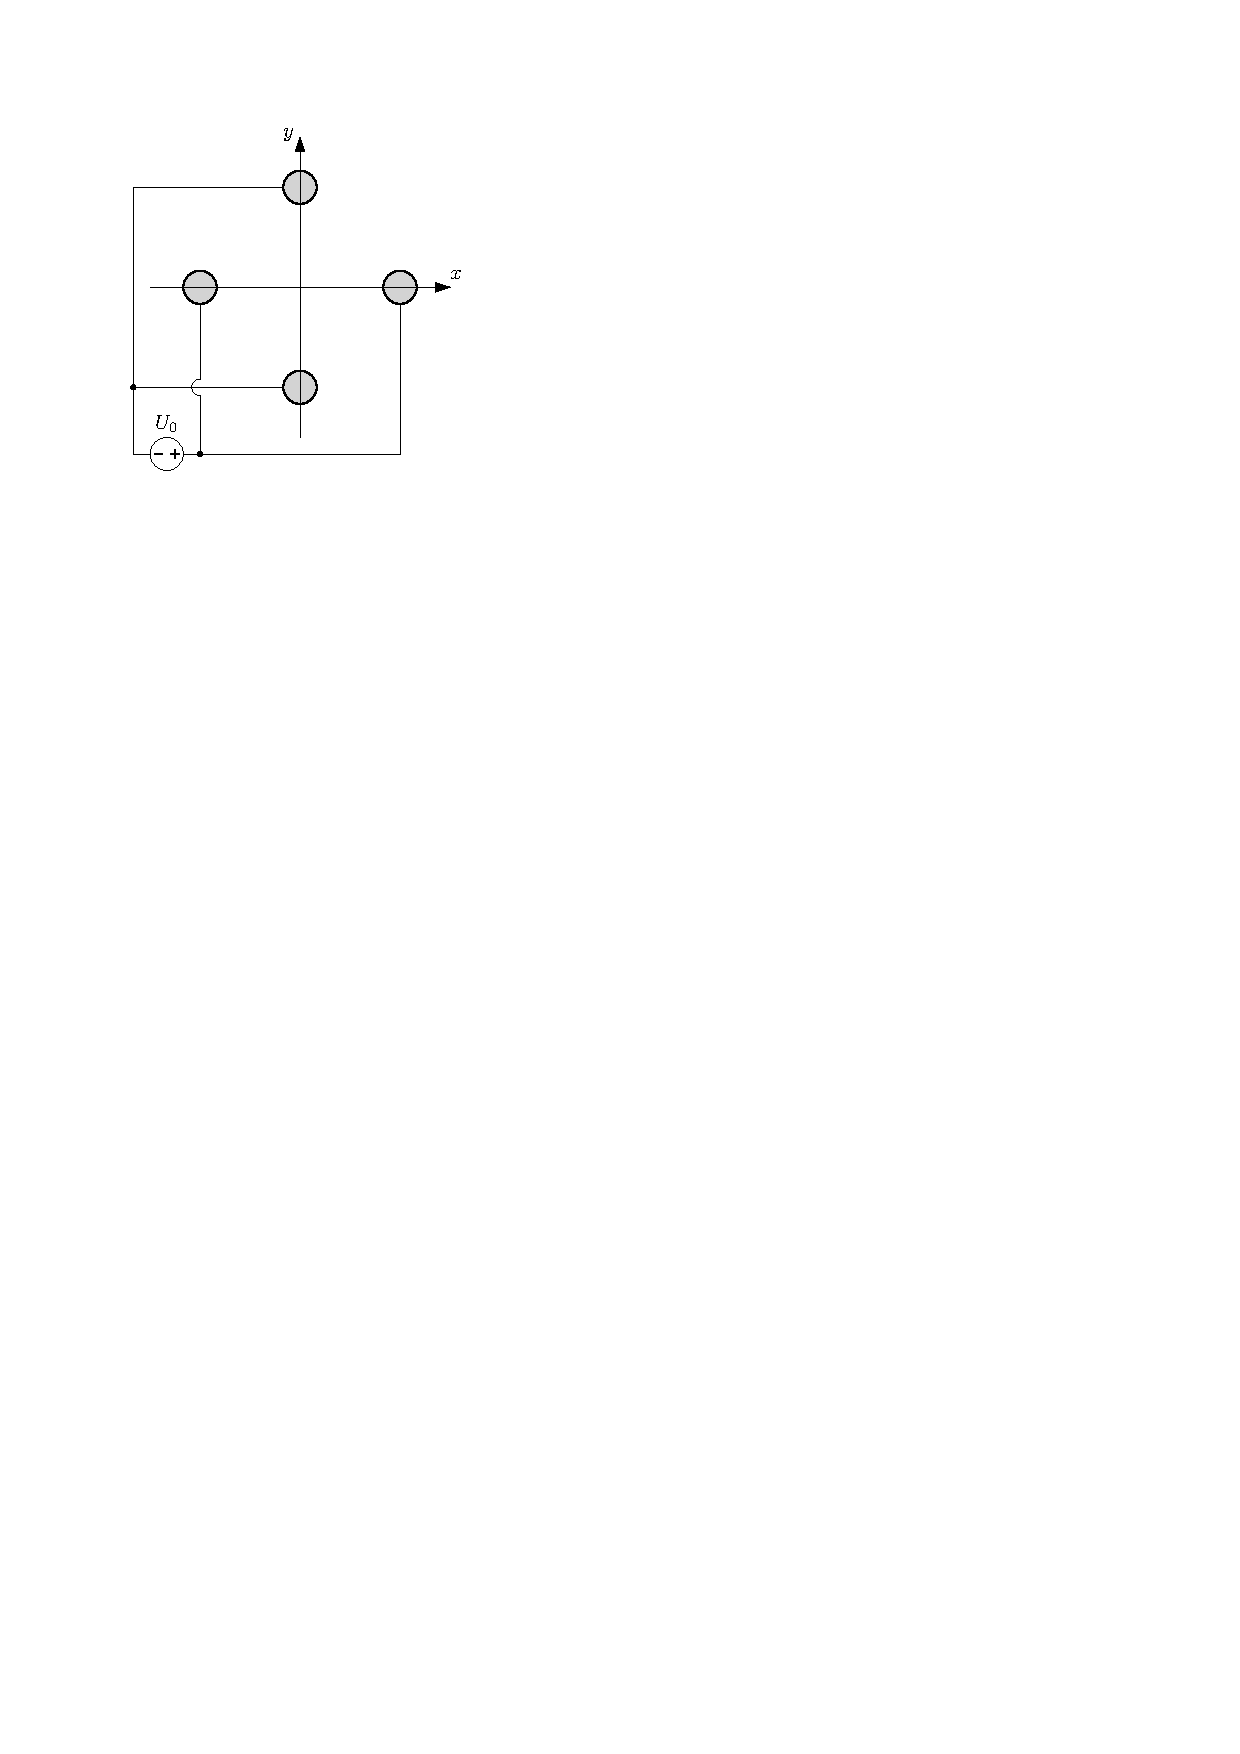
\includegraphics[width=0.8\textwidth]{./figures/lineare_paulfalle_xy_statisch.pdf}
		\end{figure}
		
		\column{0.5\textwidth}
		Quadrupol-Potential:
		\begin{align}
		\phi = \phi_0 + \frac{U_0}{2 \, r_0^2} (x^2-y^2)
		\end{align}
		\begin{figure}[h]
			\centering
			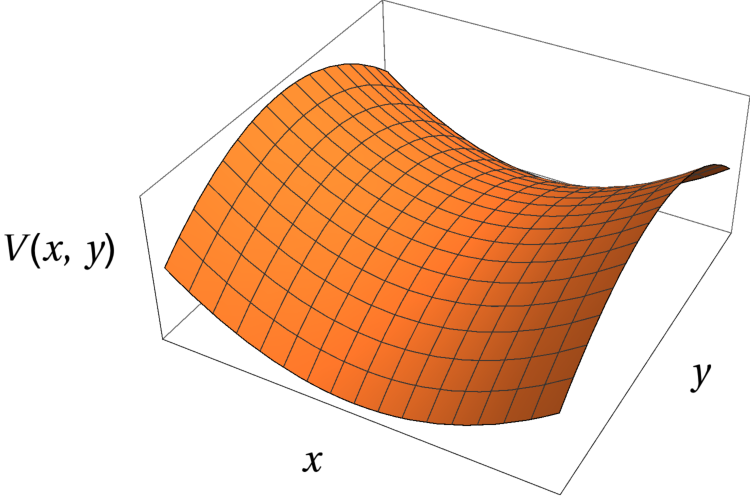
\includegraphics[width=0.95\textwidth]{./figures/sattelpotential.pdf}
		\end{figure}
	\end{columns}
\end{frame}

\begin{frame}{Lineare Paul-Falle ($x$-$y$-Ebene)}
	\begin{columns}[t]
		\column{0.5\textwidth}
		Quadrupol:
		\begin{figure}[h]
			\centering
			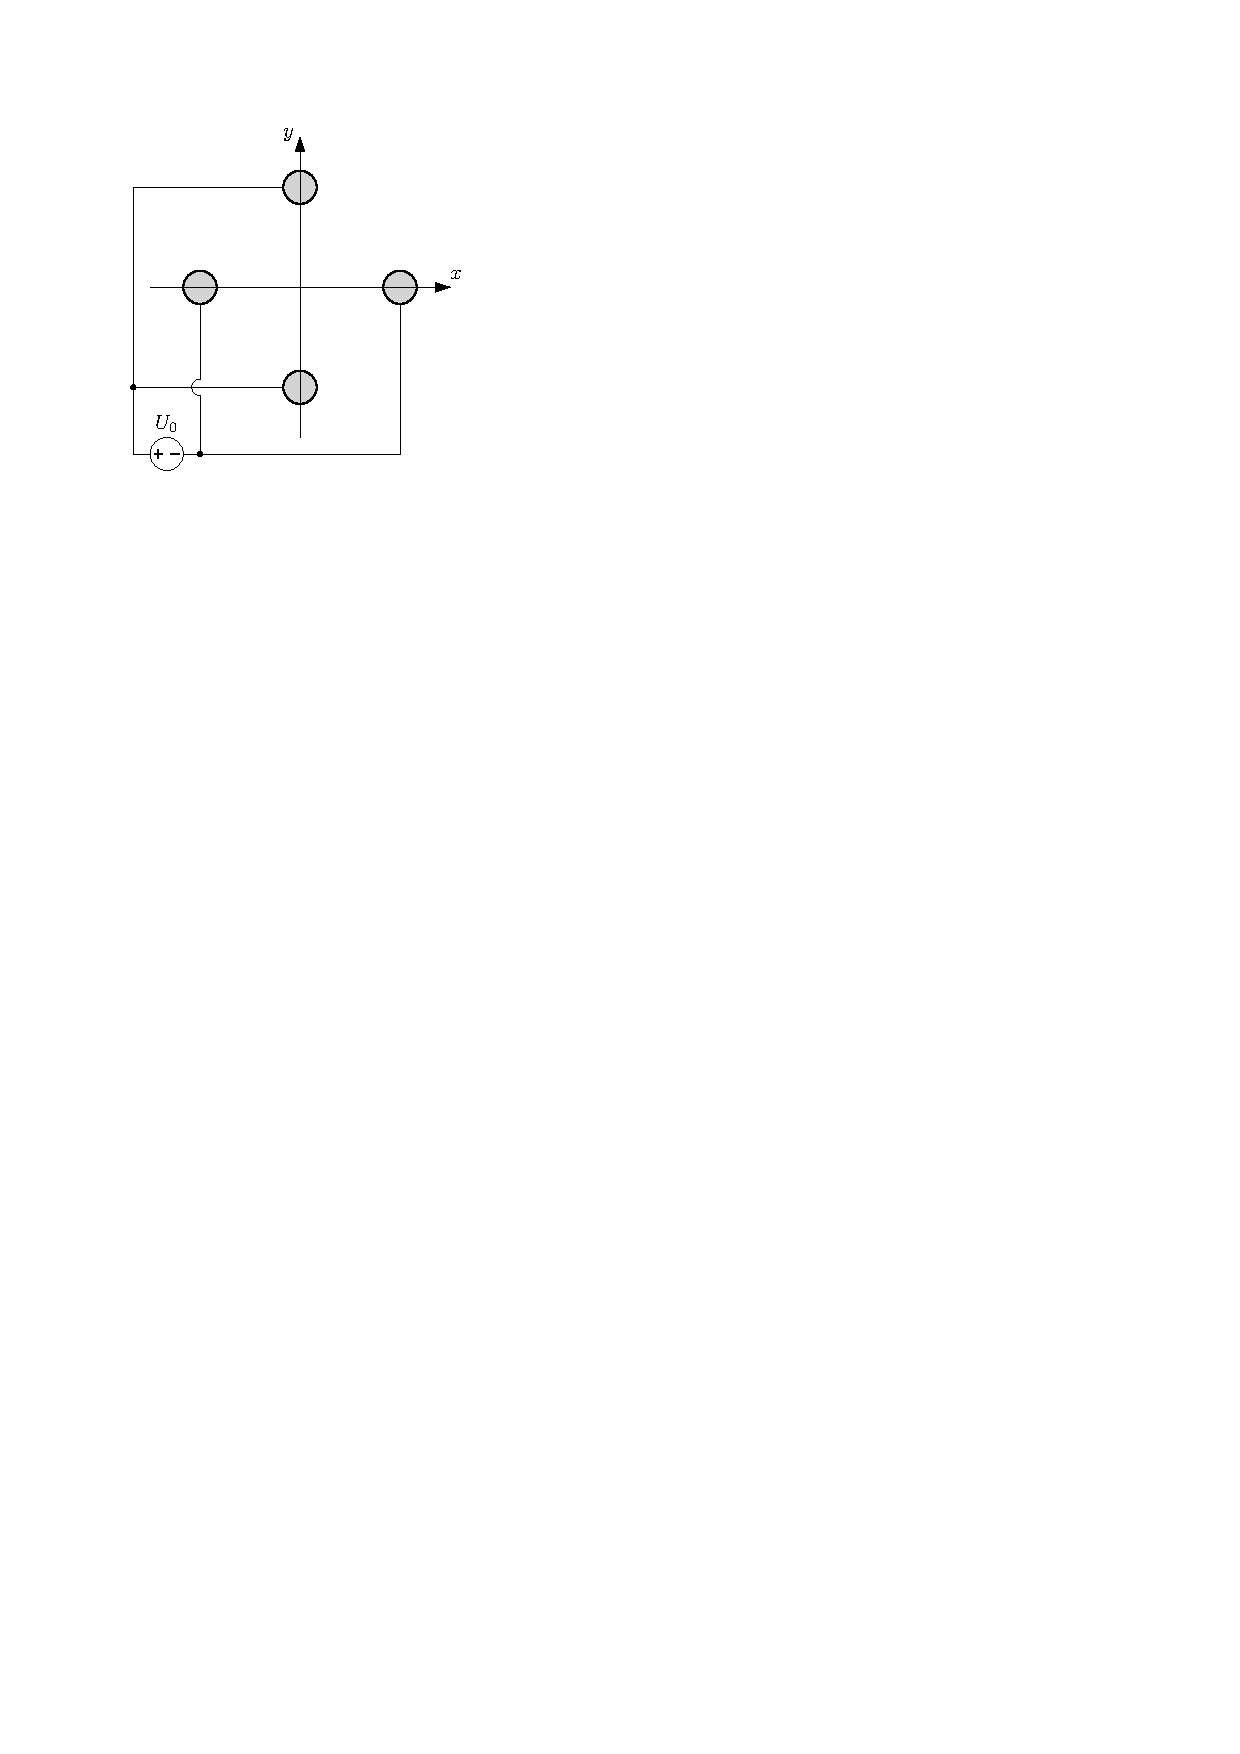
\includegraphics[width=0.8\textwidth]{./figures/lineare_paulfalle_xy_statisch_swapped.pdf}
		\end{figure}
		
		\column{0.5\textwidth}
		Quadrupol-Potential:
		\begin{align}
		\phi = \phi_0 - \frac{U_0}{2 \, r_0^2} (x^2-y^2)
		\end{align}
		\begin{figure}[h]
			\centering
			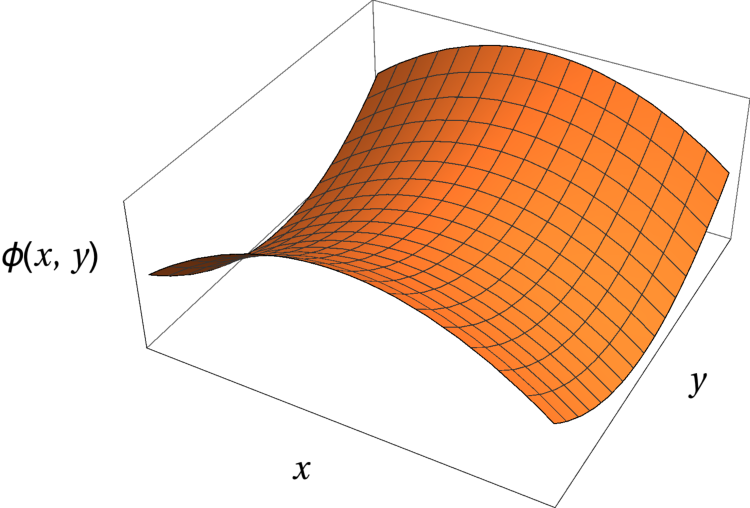
\includegraphics[width=0.95\textwidth]{./figures/sattelpotential2.pdf}
		\end{figure}
	\end{columns}
\end{frame}

\begin{frame}{Lineare Paul-Falle ($x$-$y$-Ebene)}
	Nutze Trägheit des Teilchens und verwende zeitlich variierendes Potential:
	\begin{align}
		\phi = \phi_0 + \frac{U_0}{2 \, r_0} \cos(\Omega t) \, (x^2-y^2)
	\end{align}
	Typische Frequenzen im Radiobereich $\nu = \mathcal{O}(\SI{10}{MHz})$
	
	Stabilität der Falle ist sehr sensitiv auf Ladung der Teilchen, RF-Frequenz, Feldeigenschaften und \textbf{Masse} der Teilchen
\end{frame}

\begin{frame}{Lineare Paul-Falle (Erweiterung auf die $z$-Achse)}
	\begin{columns}[t]
		\column{0.6\textwidth}
		\begin{itemize}
			\item 1
			\item 2
		\end{itemize}
		\column{0.4\textwidth}
			\begin{figure}[h]
				\centering
				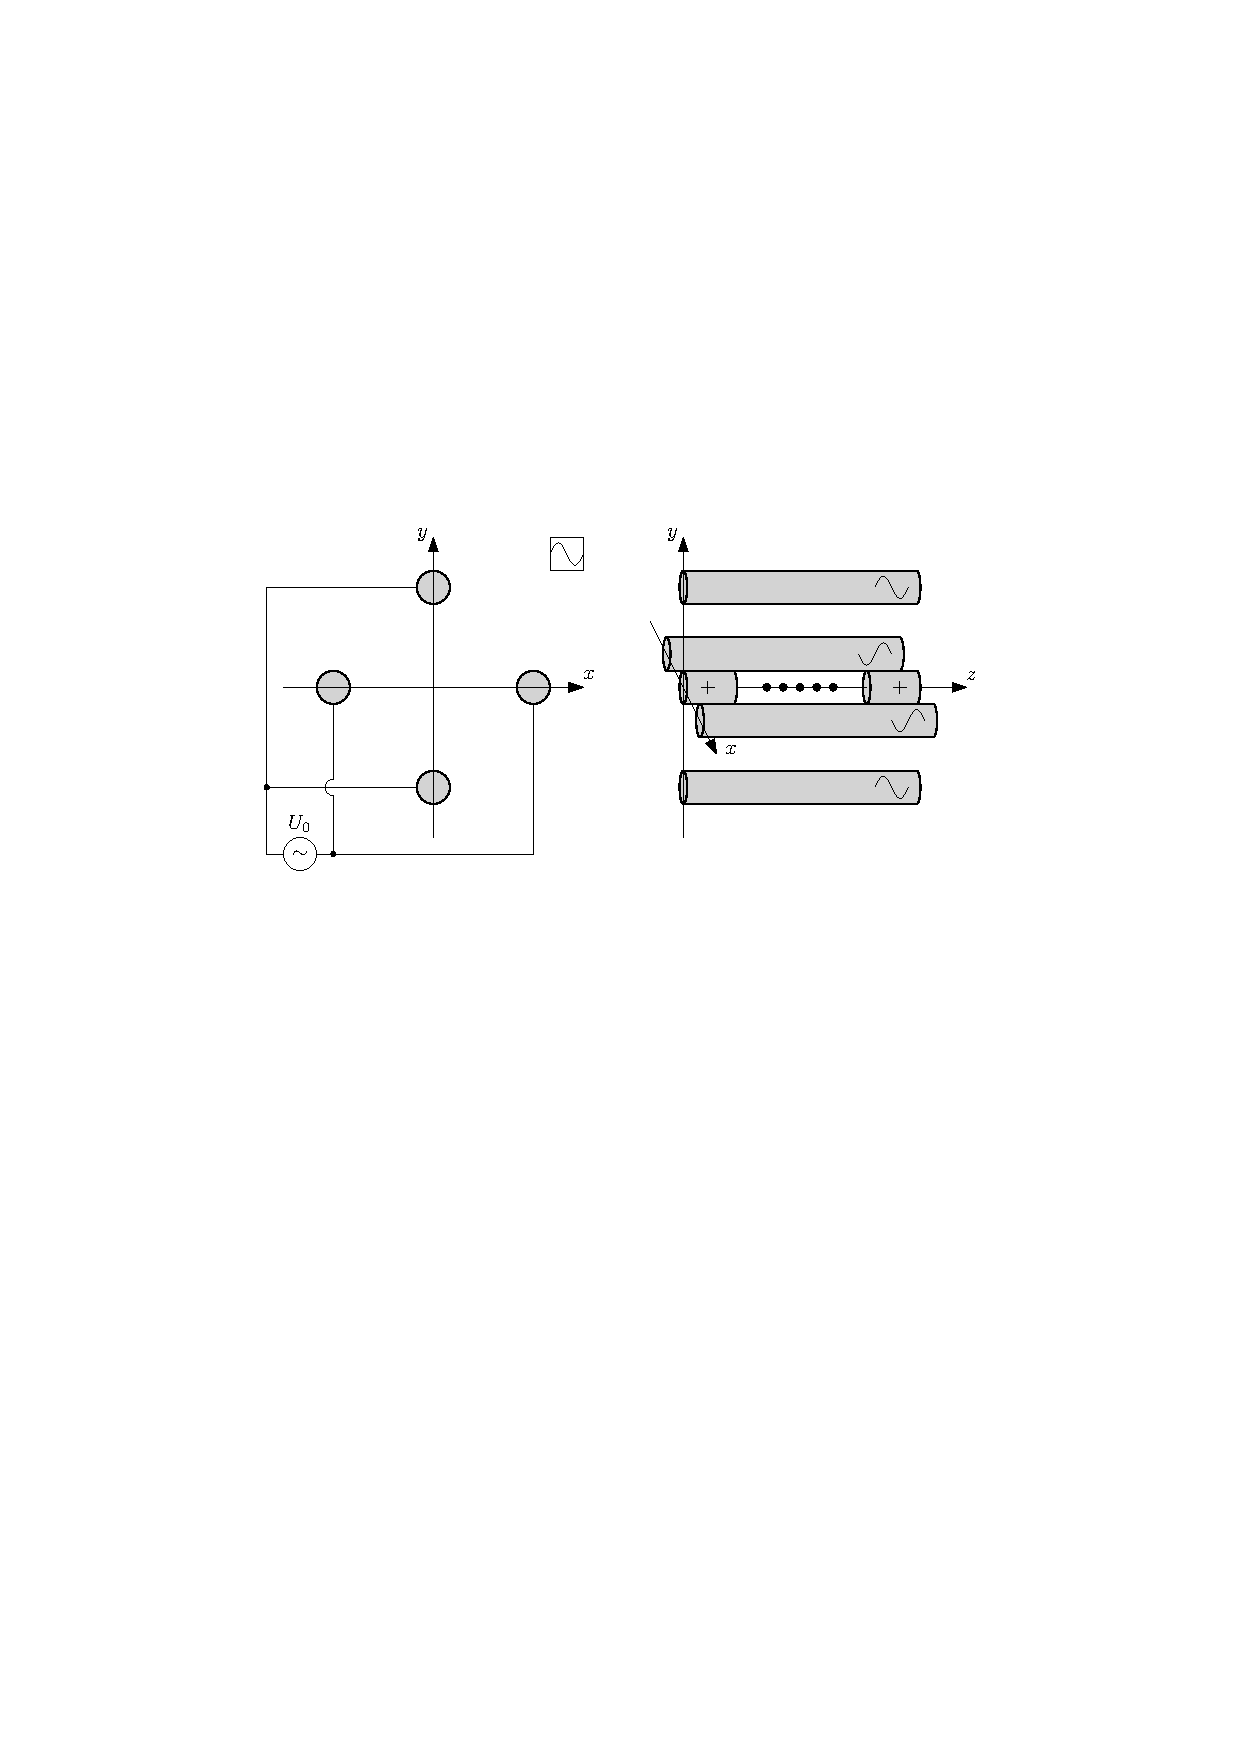
\includegraphics[width = 1\textwidth]{./figures/lineare_paulfalle.pdf}
			\end{figure}
	\end{columns}

\end{frame}

\begin{frame}{Lineare Paul-Falle}
Axiale Kraft kleiner als Radiale:
\begin{figure}[h]
	\centering
	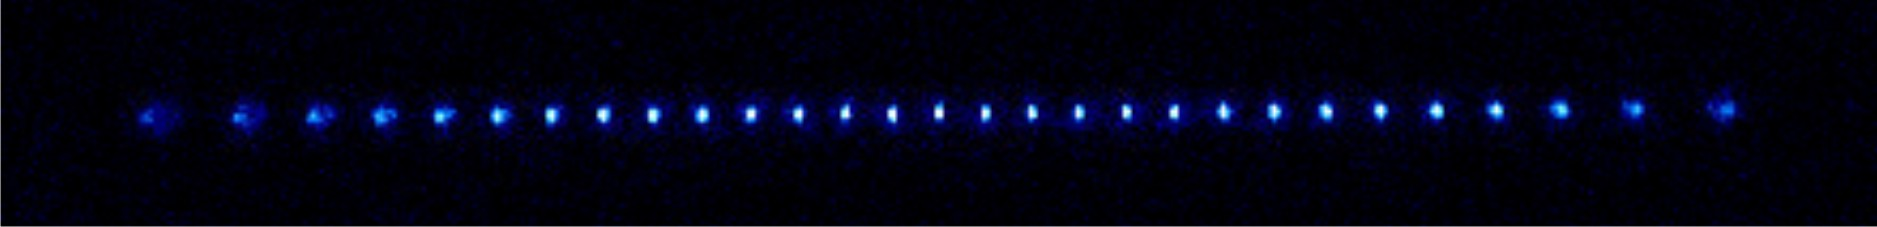
\includegraphics[width=0.9\textwidth]{./figures/29_laser_cooled_ion_chain.jpg}
	\caption{29 lasergekühlte Thorium-Atome ($\mathrm{Th}^{3+}$) in einer linearen Paul-Falle (Abstand etwa \SI{50}{\micro\metre}) \cite{campbell}}
\end{figure}

(Penning-Falle?)

\end{frame}

\section{Optische Fallen}

\begin{frame}{Einleitung}
	\begin{itemize}
		\item Fangen von neutralen Atomen
	\end{itemize}
\end{frame}

\begin{frame}{Grundlagen: Streukraft}
	\begin{columns}[t]
		\column{0.5\textwidth}
		\begin{itemize}
			\item Photonenimpuls:
			\begin{align}
			p = \frac{E}{c}
			\end{align}
			\item Absorption
			\item spontante Emission (Isotrop)
			\item mittlere (bremsende) Kraft
		\end{itemize}
		
		\column{0.5\textwidth}
		\begin{figure}[h]
			\centering
			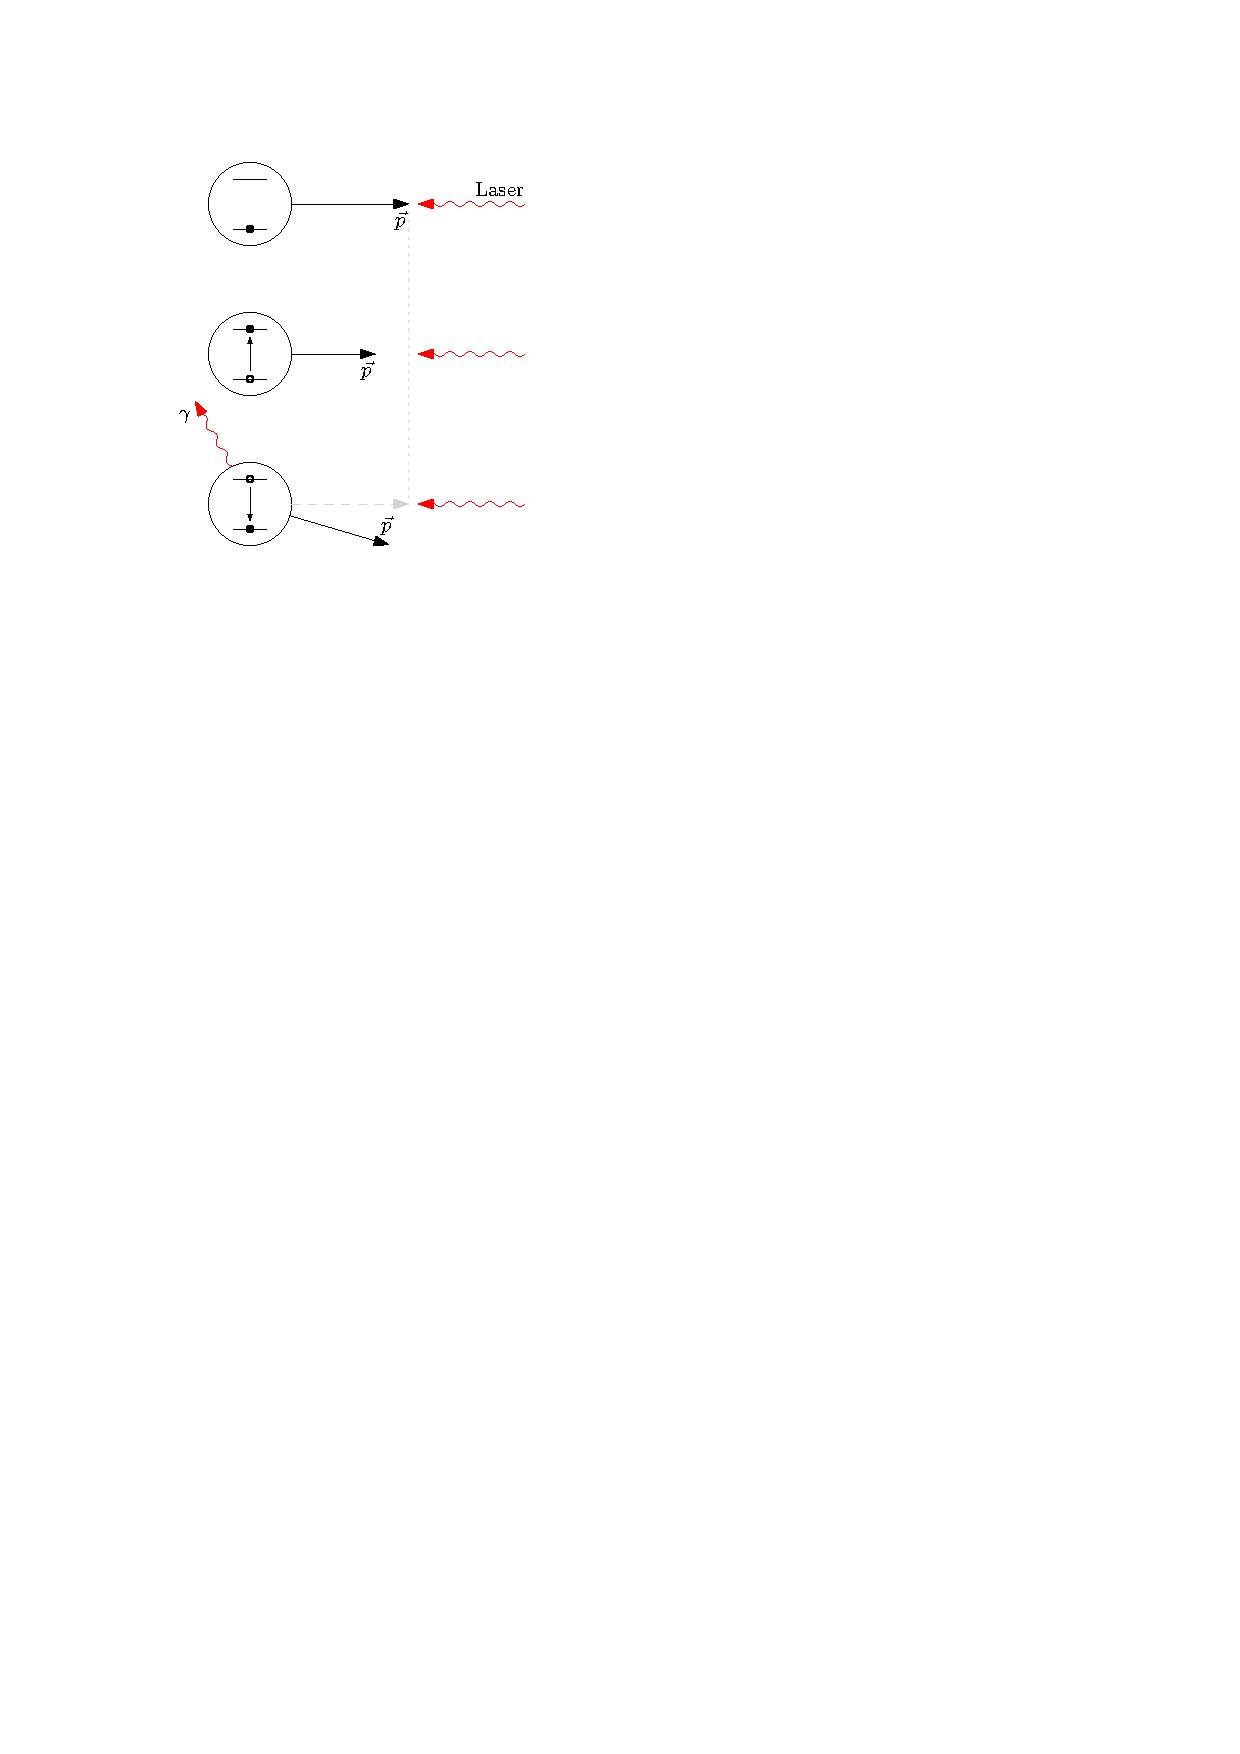
\includegraphics[width=1.0\textwidth]{./figures/streukraft.pdf}
		\end{figure}
		
	\end{columns}

\end{frame}

\begin{frame}{Optische Melasse}
\begin{figure}[h]
	\centering
	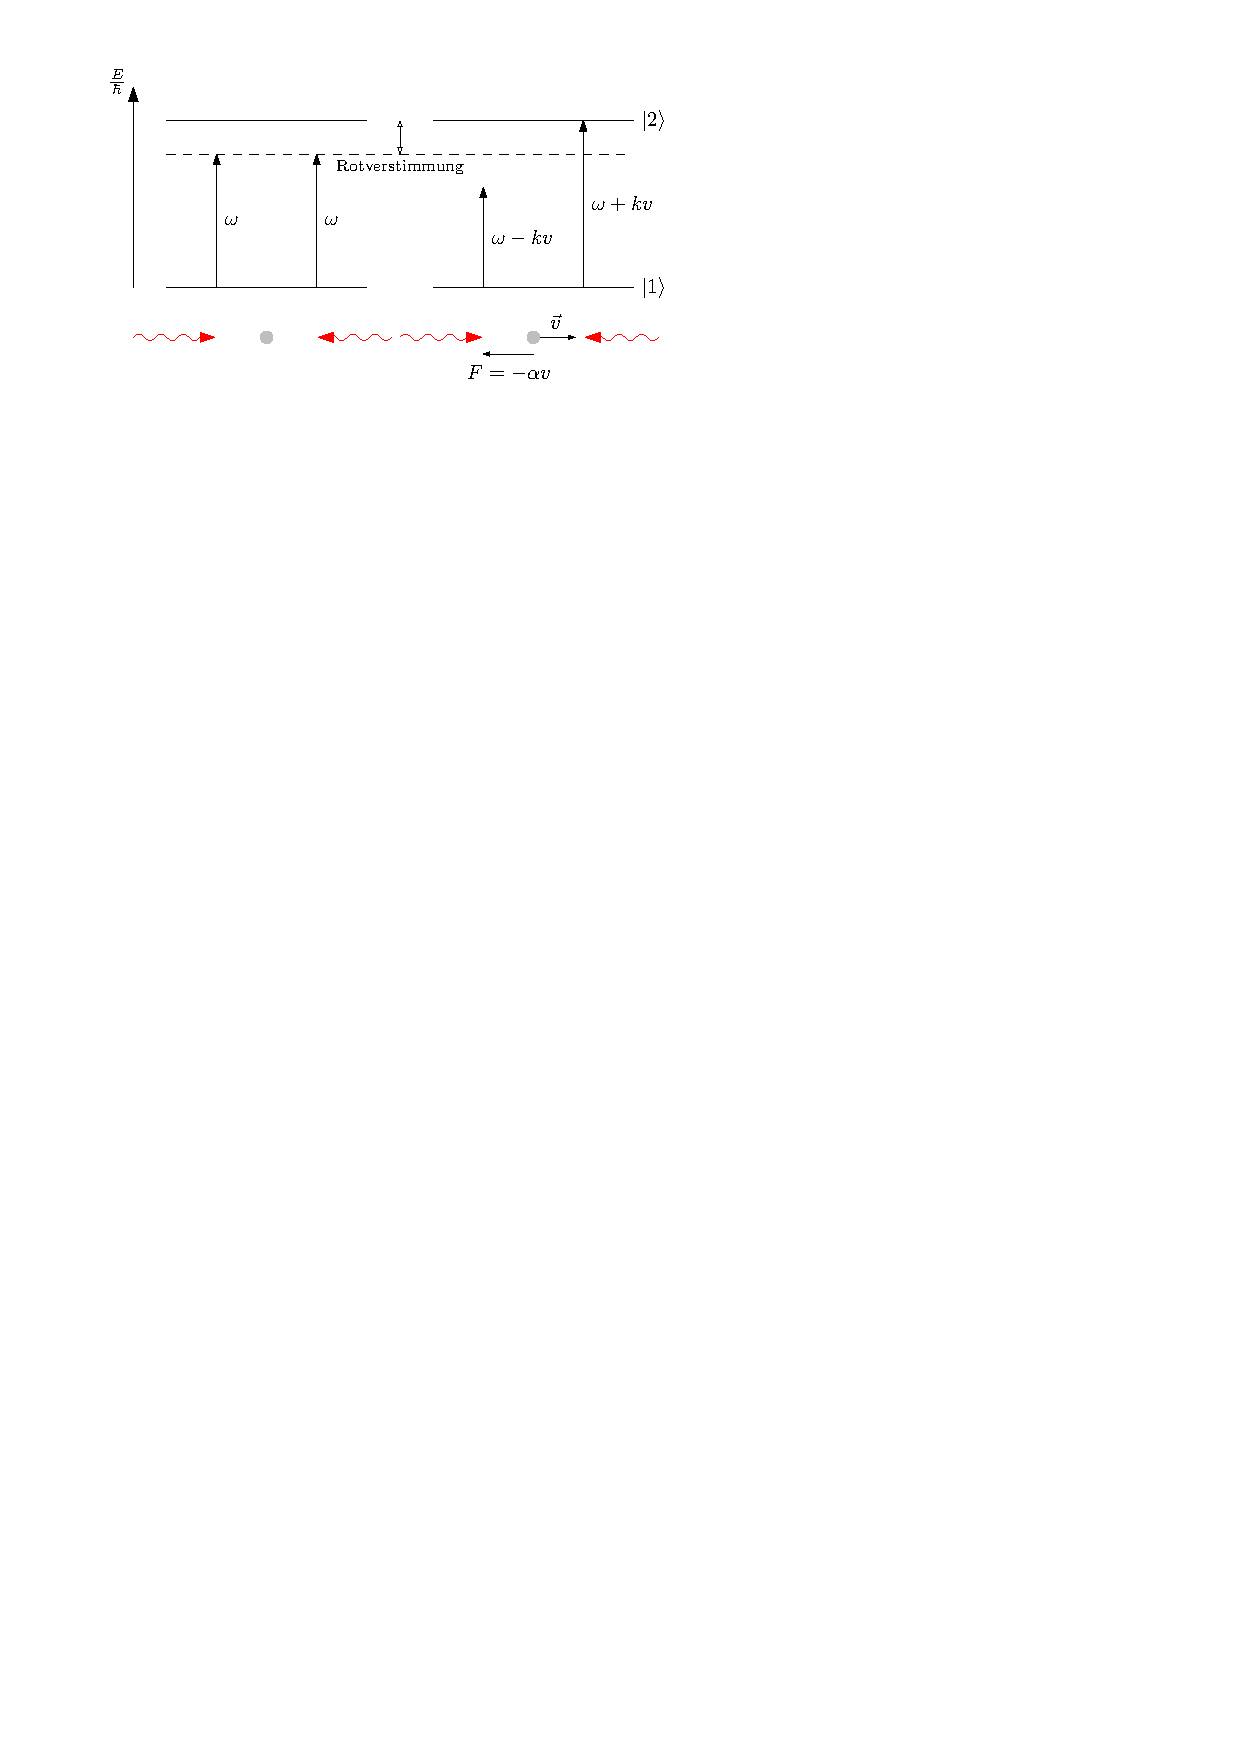
\includegraphics[width=\textwidth]{./figures/melasse.pdf}
\end{figure}
\end{frame}

\begin{frame}{Grundlagen: Feinstruktur und Zeeman-Aufspaltung}
	\begin{itemize}
		\item Ein Atom hat ein magnetisches Dipolmoment $\vec{\mu}$ aufgrund des Gesamtdrehimpulses $\vec{J}$ (Zusammengesetzt aus Bahndrehimpuls $\vec{L}$ und Spin $\vec{S}$).
		\begin{align}
		\vec{\mu} = - \frac{\mu_\mathrm{B} g_J \vec{J}}{\hbar} \quad \text{unnötig}
		\end{align}
		\item Die potentielle Energie eines magnetischen Dipols im homogenen Magnetfeld ist gegeben durch:
		\begin{align}
		V = - \vec{\mu} \cdot \vec{B}
		\end{align}
		\item Im externen Magnetfeld $\vec{B}$ führt dies zu einer Aufspaltung der Energieniveaus:
		\begin{align}
		\Delta E = \mu_\mathrm{B} \, g_J \, m_J \, B
		\end{align}
	\end{itemize}
\end{frame}

\begin{frame}{Magneto-optische Falle}
\SI{1}{K} tief

\begin{figure}[h]
	\centering
	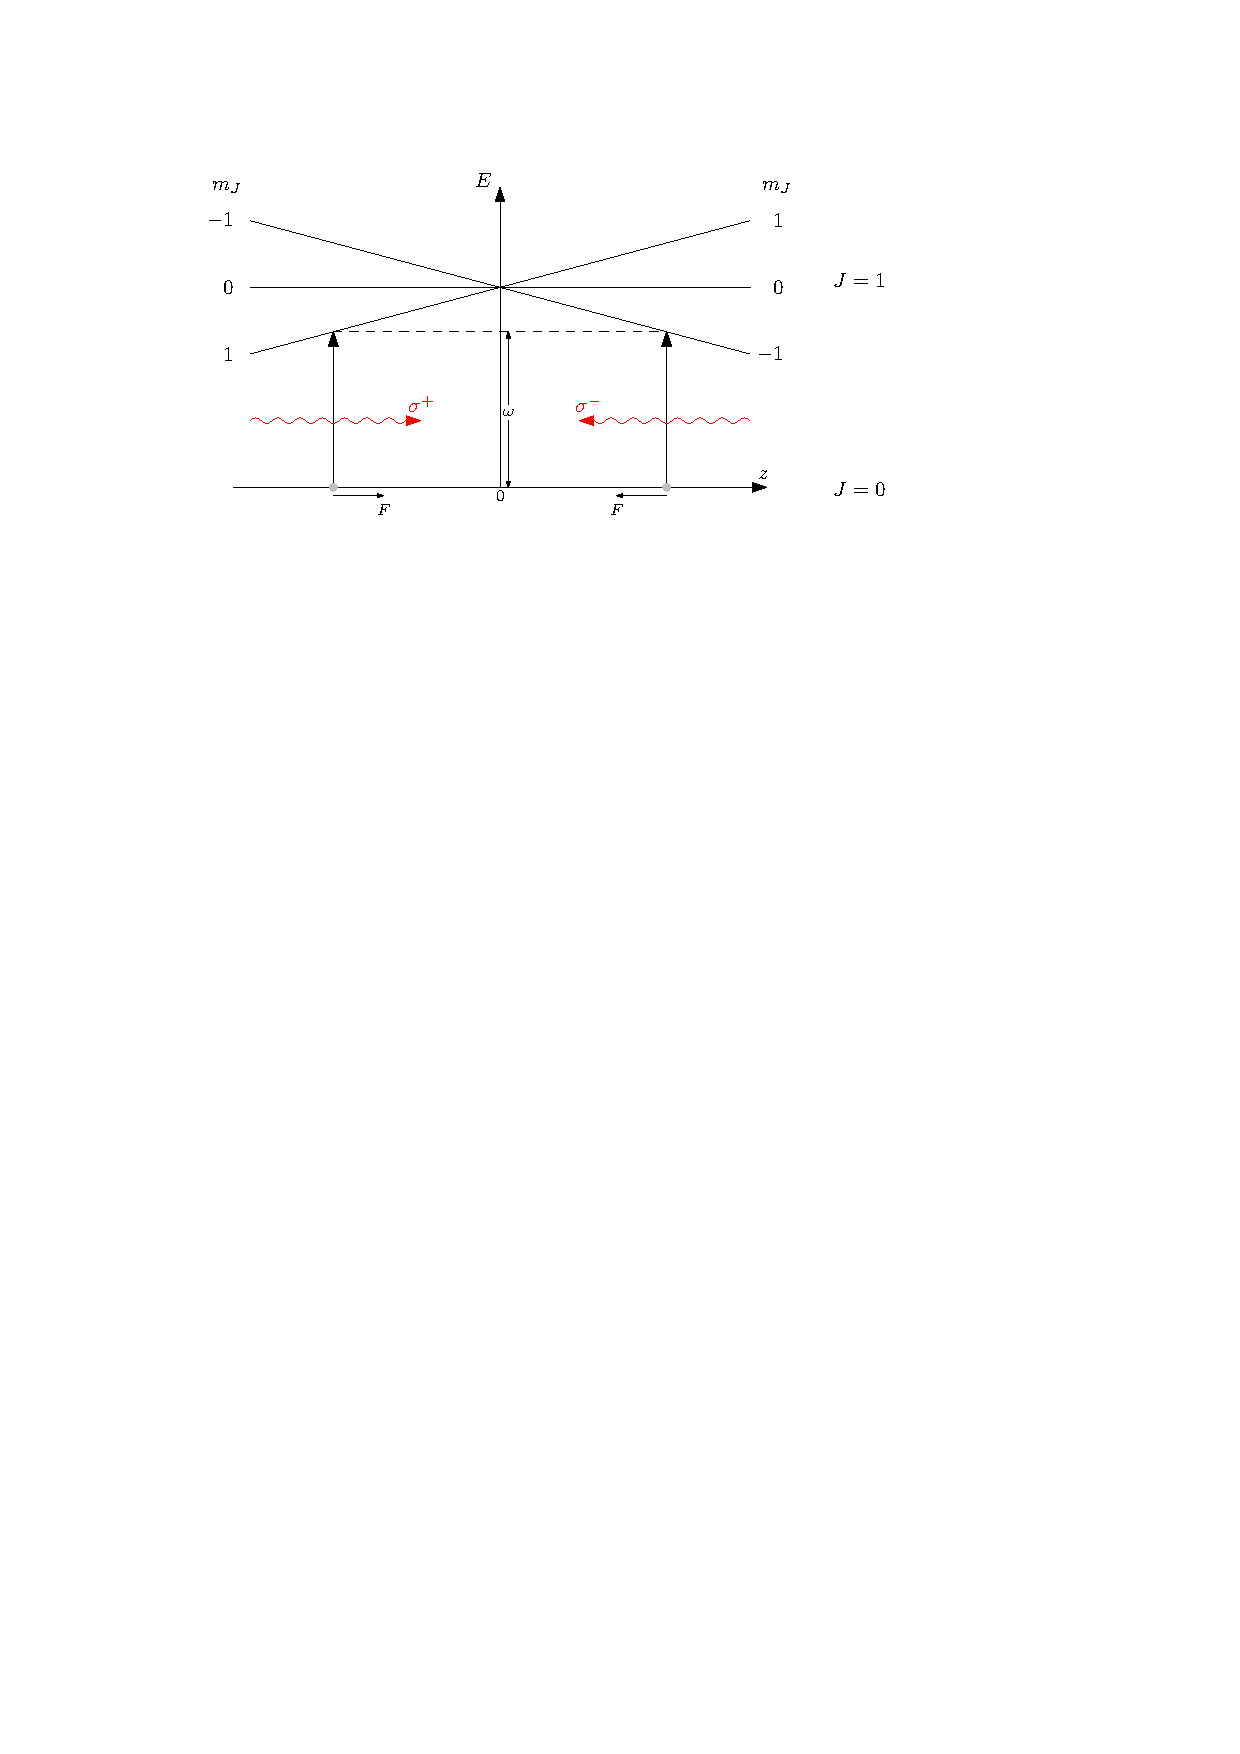
\includegraphics[width=0.8\textwidth]{./figures/mot.pdf}
\end{figure}
\end{frame}

\begin{frame}{MOT}
	\begin{itemize}
		\item Magnetfeld
		\item typischer Versuchsablauf: MOT beladen durch atomischen Strahl (Zeeman-Slower), MOT wird abgeschaltet damit durch optische Melasse gekühlt wird (Zeeman-Effekt hat negativen Einfluss auf Dopplerkühlung)
		\item In einer gefüllten Falle kommt es zur ständigen Streuung des Laserlichts, was mit dem Auge/CCD sichtbar ist
		\item Gebraucht zum Laden von Dipolfallen/Magnetfallen
		\item typisches Magnetfeld \SI{0.1}{\tesla\per\metre}
	\end{itemize}
\end{frame}

\begin{frame}{Dipol-Falle (opt. Pinzette) (?)}
\end{frame}


\section{Magnetfalle}

\begin{frame}{Magnetfalle}
typische Fallentiefe: \SI{0.07}{\kelvin}
Majorana Übergang!
\end{frame}


\section{Vergleich}

\begin{frame}{Fallentiefen}
	\begin{table}
	\begin{tabular}{l | c | c | c }
		& Paul-Falle & MOT & Magnetfalle \\
		\hline
		Fallentiefe & \SI{1}{K} & \SI{1}{K} & \SI{1}{K} \\
		Vorteile & & & \\
		Nachteile & & & \\
		Lebenszeit & & & \\
	\end{tabular}
	\end{table}

\end{frame}

\begin{frame}{Vielen Dank für die Aufmerksamkeit}
\end{frame}

\section{Literatur}

\begin{frame}{Literatur}
	\begin{thebibliography}{9}
		\bibitem{foot}
		Christopher J. Foot,
		\emph{Atomic Physics},
		Oxford University Press 2005
		
		\bibitem{campbell}
		Corey J. Campbell,
		\emph{Trapping, Laser Cooling, and Spectroscopy of Thorium IV},
		Georgia Institute of Technlogy 2011
		
		\bibitem{wpw}
		Carl E. Wieman, David E. Pritchard, David J. Wineland,
		\emph{Atom cooling, trapping, and quantum manipulation},
		Reviews of Modern Physics, Vol. 71, No.2 1999
		
	\end{thebibliography}
	
\end{frame}

\end{document}